%%%%%%%%%%%%%%%%%%%%%%%%%%%%%%%%%%%%%%%%%%%%%%%%%%%%%%%%%%%%%%%%%%%%%%%%%%%%%%%%%%
\begin{frame}[fragile]\frametitle{}
\begin{center}
{\Large Fine-tuning GPT}
\end{center}
\end{frame}

%%%%%%%%%%%%%%%%%%%%%%%%%%%%%%%%%%%%%%%%%%%%%%%%%%%%%%%%%%%
\begin{frame}[fragile]\frametitle{Fine-tuning GPT}

\begin{center}
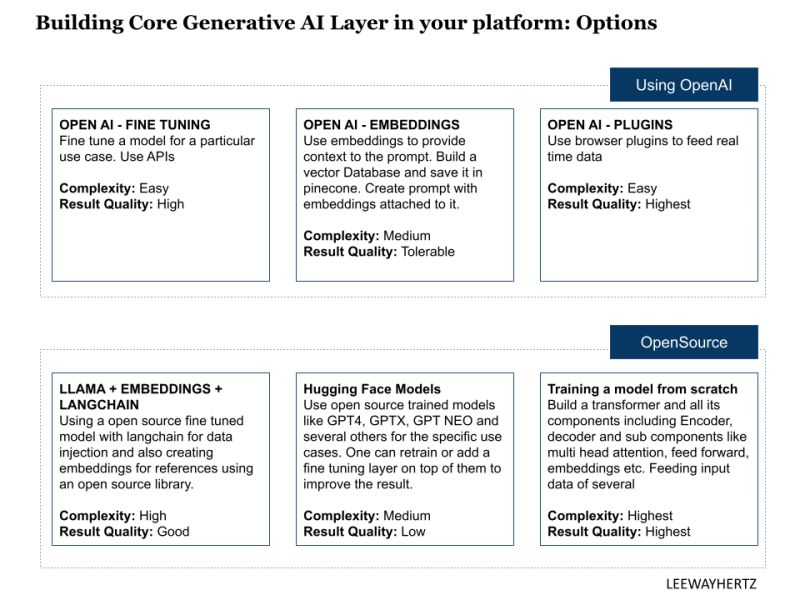
\includegraphics[width=\linewidth,keepaspectratio]{promptengg29}

{\tiny (Ref: LinkedIn post by Akash Takyar )}

\end{center}		


\end{frame}

%%%%%%%%%%%%%%%%%%%%%%%%%%%%%%%%%%%%%%%%%%%%%%%%%%%%%%%%%%%
\begin{frame}[fragile]\frametitle{Fine-tuning GPT}

\begin{center}
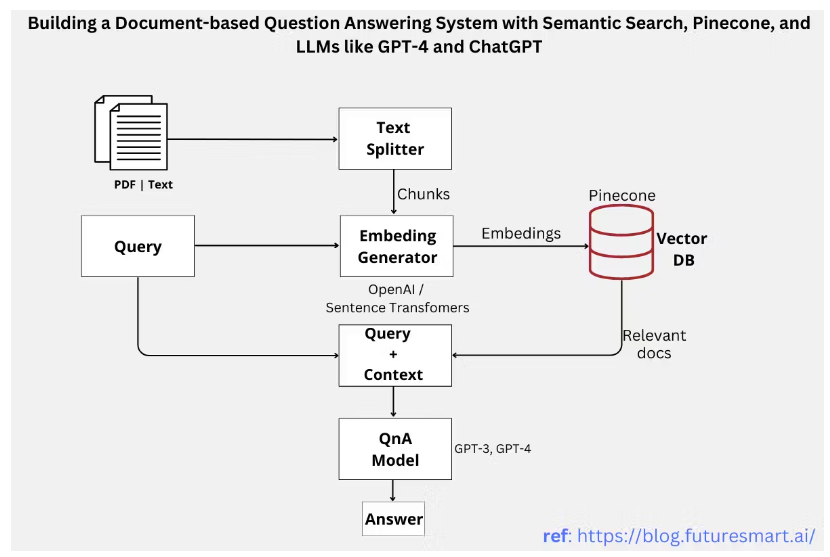
\includegraphics[width=\linewidth,keepaspectratio]{langchain6}

{\tiny (Ref: FutureSmart AI Blog)}

\end{center}		


\end{frame}


%%%%%%%%%%%%%%%%%%%%%%%%%%%%%%%%%%%%%%%%%%%%%%%%%%%%%%%%%%%%%%%%%%%%%%%%%%%%%%%%%%
\begin{frame}[fragile]\frametitle{}
\begin{center}
{\Large Custom ChatGPT with Azure OpenAI \\ by Valentina Alto}

{\tiny (Ref: code at https://github.com/AI-Yash/st-chat)}

\end{center}
\end{frame}

%%%%%%%%%%%%%%%%%%%%%%%%%%%%%%%%%%%%%%%%%%%%%%%%%%%%%%%%%%%
\begin{frame}[fragile]\frametitle{ Background}


\begin{itemize}
\item Customizing ChatGPT directly is not available as of now.
\item But, can leverage ChatGPT backend model, the GPT3, via REST API or Python SDK and embed them into their application.
\item Additionally, since the General Availability of Azure OpenAI Service, the very same models are also available as a service in the Azure cloud, benefiting from scalability, flexibility, security, and built-in responsible AI.
\item Using  \lstinline|Streamlit|, an open-source Python library that makes it easy to create and deploy interactive web applications for machine learning, data science, and other data-driven tasks. (More specifically, we are going to use a component \lstinline|streamlit-chat|)
\end{itemize}	 

\end{frame}

%%%%%%%%%%%%%%%%%%%%%%%%%%%%%%%%%%%%%%%%%%%%%%%%%%%%%%%%%%%
\begin{frame}[fragile]\frametitle{ Requirements}

\begin{itemize}
\item An Azure subscription — Create one for free at https://azure.microsoft.com/free/cognitive-services
\item Ask access to Azure OpenAI in the desired Azure subscription https://aka.ms/oai/access
\item Python 3.7.1 or later version
\item An Azure OpenAI Service resource for model deployment
\end{itemize}	 

\end{frame}

%%%%%%%%%%%%%%%%%%%%%%%%%%%%%%%%%%%%%%%%%%%%%%%%%%%%%%%%%%%
\begin{frame}[fragile]\frametitle{ Setup Open AI}

All the OpenAI variables can be found within your Azure OpenAI instance, under ``Keys and Endpoint''.

\begin{lstlisting}
import toml

with open('secrets.toml', 'r') as f:
    config = toml.load(f)

openai.api_type = "azure"
openai.api_key = config['OPENAI_API_KEY']
openai.api_base = "https://openaitest123.openai.azure.com/"
openai.api_version = "2022-12-01"

\end{lstlisting}	 


\end{frame}

%%%%%%%%%%%%%%%%%%%%%%%%%%%%%%%%%%%%%%%%%%%%%%%%%%%%%%%%%%%
\begin{frame}[fragile]\frametitle{ Setup Open AI}

\begin{center}
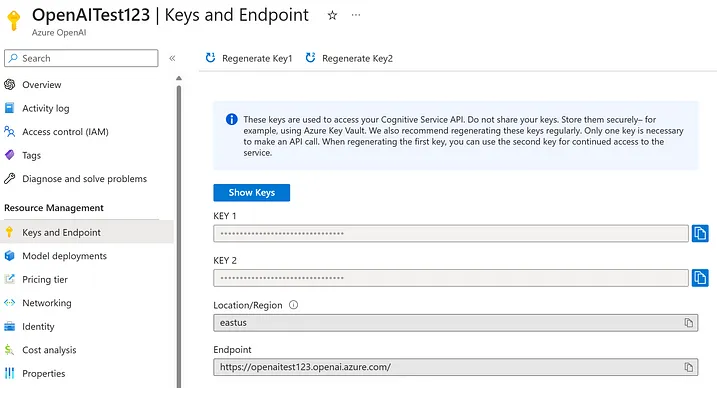
\includegraphics[width=\linewidth,keepaspectratio]{chatgpt38}
\end{center}

\end{frame}

%%%%%%%%%%%%%%%%%%%%%%%%%%%%%%%%%%%%%%%%%%%%%%%%%%%%%%%%%%%
\begin{frame}[fragile]\frametitle{ Setup streamlit-chat }

\begin{lstlisting}
import streamlit as st
from streamlit_chat import message
import requests
import openai

st.set_page_config(page_title="Custom ChatGPT")

st.markdown("# Custom ChatGPT")
st.sidebar.header("Custom ChatGPT")

#generating 2 empty lists to store past and generated value in the conversation

if 'generated' not in st.session_state:
    st.session_state['generated'] = []

if 'past' not in st.session_state:
    st.session_state['past'] = []

\end{lstlisting}	 

\end{frame}

%%%%%%%%%%%%%%%%%%%%%%%%%%%%%%%%%%%%%%%%%%%%%%%%%%%%%%%%%%%
\begin{frame}[fragile]\frametitle{API call }
We are leveraging our Azure OpenAI deployments (associated to a davinci model) to process the message generated by the user.


\begin{lstlisting}
user_input = st.text_input("You: ","Hello, how are you?", key="input")
if user_input:
    output = openai.Completion.create(
          engine="test1",
          prompt=user_input,
          temperature=0,
          max_tokens=1041,
          top_p=1,
          frequency_penalty=0,
          presence_penalty=0,
          best_of=1,
          stop=None)
    st.session_state.past.append(user_input)
    st.session_state.generated.append(output["choices"][0]["text"].strip())
		
if st.session_state['generated']:
    for i in range(len(st.session_state['generated'])-1, -1, -1):
        message(st.session_state["generated"][i], avatar_style = 'bottts', key=str(i))
        message(st.session_state['past'][i], avatar_style = 'big-ears',is_user=True, key=str(i) + '_user')		
\end{lstlisting}	 


\end{frame}

%%%%%%%%%%%%%%%%%%%%%%%%%%%%%%%%%%%%%%%%%%%%%%%%%%%%%%%%%%%
\begin{frame}[fragile]\frametitle{ Run}
 Save the .py file and run it via the terminal command \lstinline|streamlit run file.py|.

\begin{center}
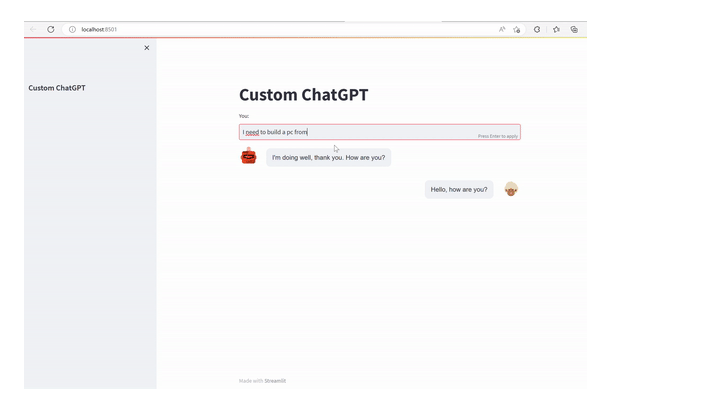
\includegraphics[width=0.8\linewidth,keepaspectratio]{chatgpt39}
\end{center}

\end{frame}

%%%%%%%%%%%%%%%%%%%%%%%%%%%%%%%%%%%%%%%%%%%%%%%%%%%%%%%%%%%
\begin{frame}[fragile]\frametitle{Memory}

Leverage learning from the context and keeping the memory of previous conversations. As you can see, now we are providing our model not only with user input but also with the previous conversation as context. 


\begin{lstlisting}
if user_input:
    output = openai.Completion.create(
          engine="test1",
          prompt=f"{st.session_state.past}\n{user_input}",
          temperature=0,
          max_tokens=1041,
          top_p=1,
          frequency_penalty=0,
          presence_penalty=0,
          best_of=1,
          stop=None)

    st.session_state.past.append(user_input)
    st.session_state.generated.append(output["choices"][0]["text"].strip())
\end{lstlisting}	 


\end{frame}


%%%%%%%%%%%%%%%%%%%%%%%%%%%%%%%%%%%%%%%%%%%%%%%%%%%%%%%%%%%
\begin{frame}[fragile]\frametitle{ Run}
 Save the .py file and run it via the terminal command \lstinline|streamlit run file.py|.

\begin{center}
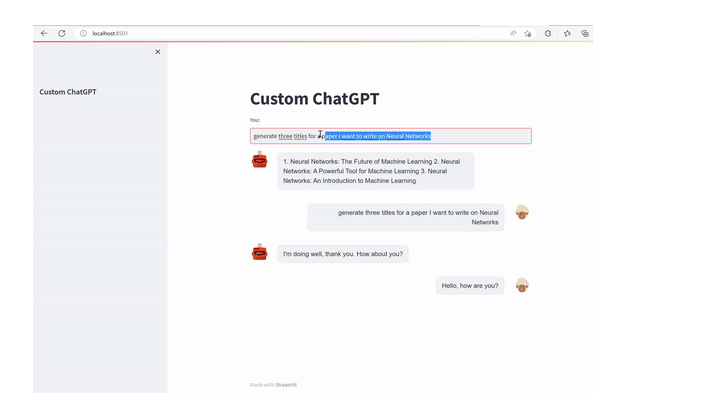
\includegraphics[width=0.8\linewidth,keepaspectratio]{chatgpt40}
\end{center}

Nice! Our custom ChatGPT kept memory about its previous answer, knowing what “title 2” refers to.

\end{frame}

%%%%%%%%%%%%%%%%%%%%%%%%%%%%%%%%%%%%%%%%%%%%%%%%%%%%%%%%%%%%%%%%%%%%%%%%%%%%%%%%%%
\begin{frame}[fragile]\frametitle{}
\begin{center}
{\Large GPT-3 Custom Training}
\end{center}
\end{frame}

%%%%%%%%%%%%%%%%%%%%%%%%%%%%%%%%%%%%%%%%%%%%%%%%%%%%%%%%%%%%%%%%%%%%%%%%%%%%%%%%%%
\begin{frame}[fragile]\frametitle{}
\begin{center}
{\Large Build your own Q\&A KnowledgeBot using GPT-Index \& LangChain - Document to Chatbot\\ 1littlecoder}
\end{center}
\end{frame}

%%%%%%%%%%%%%%%%%%%%%%%%%%%%%%%%%%%%%%%%%%%%%%%%%%%%%%%%%%%
\begin{frame}[fragile]\frametitle{Intro}

\begin{center}
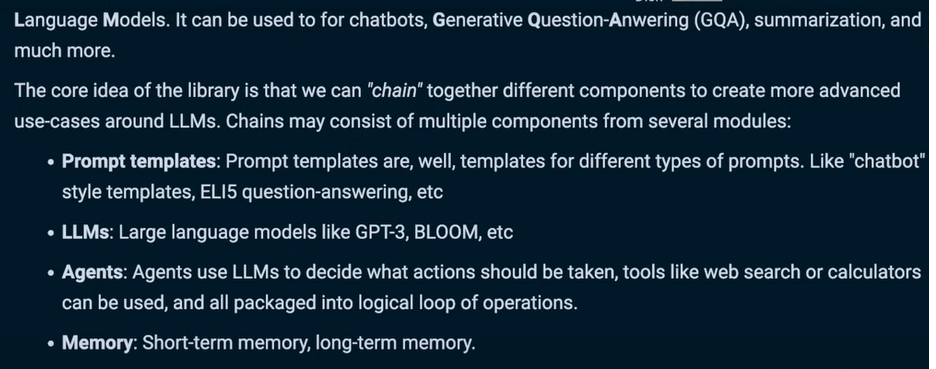
\includegraphics[width=\linewidth,keepaspectratio]{chatgpt43}

{\tiny (Ref: Getting Started with GPT-3 vs. Open Source LLMs - James Briggs)}

\end{center}		


\end{frame}

%%%%%%%%%%%%%%%%%%%%%%%%%%%%%%%%%%%%%%%%%%%%%%%%%%%%%%%%%%%
\begin{frame}[fragile]\frametitle{ Architecture}

\begin{center}
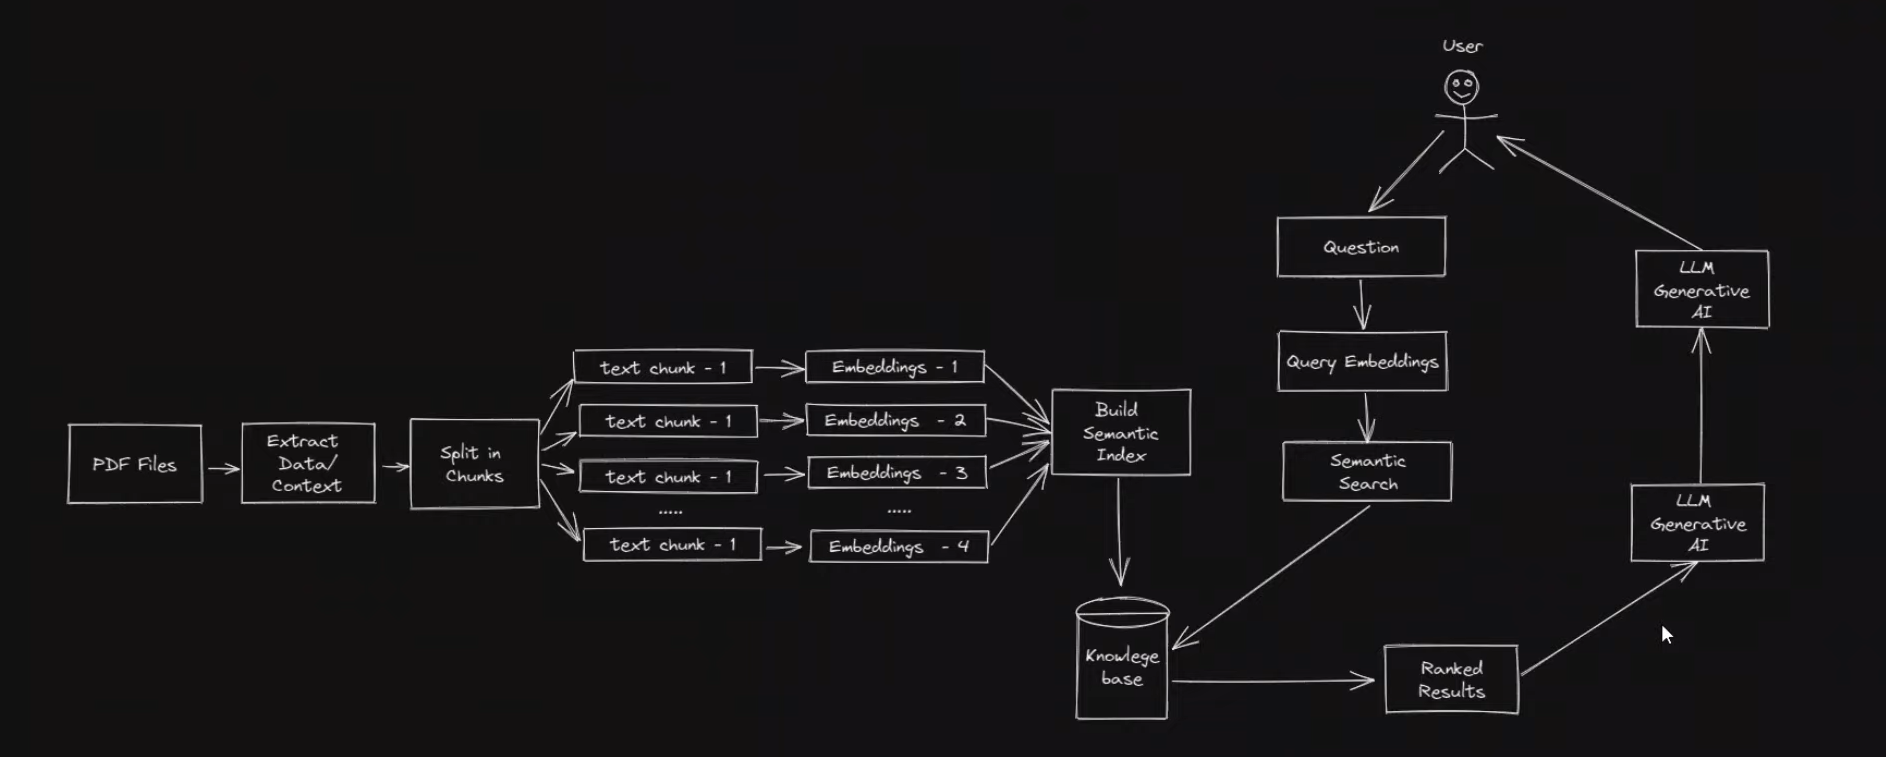
\includegraphics[width=\linewidth,keepaspectratio]{chatgpt44}

{\tiny (Ref: ChatGPT for YOUR OWN PDF files with LangChain - Prompt Engineering)}

\end{center}

\end{frame}


%%%%%%%%%%%%%%%%%%%%%%%%%%%%%%%%%%%%%%%%%%%%%%%%%%%%%%%%%%%
\begin{frame}[fragile]\frametitle{Contours}

\begin{itemize}
\item Input: some txt file, say of book `Meditations` by Marcus Aurelius
\item Goal: to build a chatbot to answer questions related to the book.
\item Usage: FAQ chatbot, based on QnA bank.
\item Method: LangChain (https://github.com/hwchase17/langchain) to access OpenAI model and GPT-index (https://github.com/jerryjliu/llama\_index) to build the vector search, to create embedding of given documents.
\end{itemize}	 

{\tiny (Ref: Colab https://colab.research.google.com/drive/1JYTczk-4D86XNn0GTaXux5yi2-LfoIPd?usp=sharing)}

\end{frame}

%%%%%%%%%%%%%%%%%%%%%%%%%%%%%%%%%%%%%%%%%%%%%%%%%%%%%%%%%%%
\begin{frame}[fragile]\frametitle{Architecture}

\begin{center}
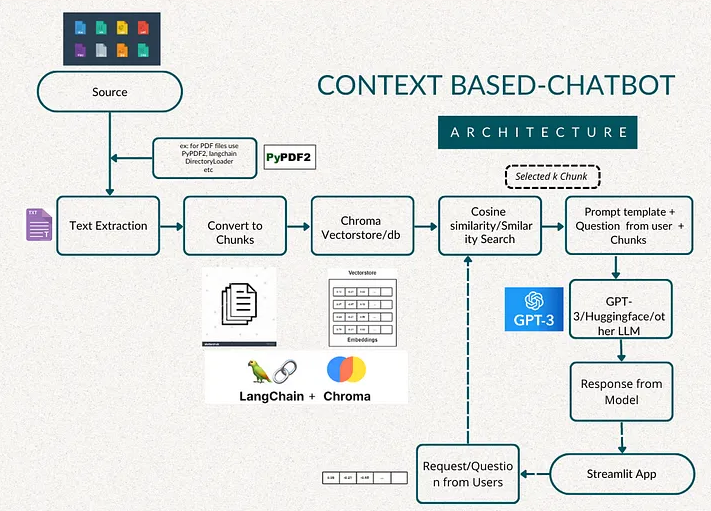
\includegraphics[width=\linewidth,keepaspectratio]{chatgpt45}

{\tiny (Ref: Document based LLM-Powered Chatbot - Abonia Sojasingarayar)}

\end{center}		


\end{frame}


%%%%%%%%%%%%%%%%%%%%%%%%%%%%%%%%%%%%%%%%%%%%%%%%%%%%%%%%%%%
\begin{frame}[fragile]\frametitle{Setup}


\begin{lstlisting}
!pip install gpt_index
!pip install langchain

!wget http://classics.mit.edu/Antoninus/meditations.mb.txt # save it to directory_path

from gpt_index import SimpleDirectoryReader, GPTListIndex, GPTSimpleVectorIndex, LLMPredictor, PromptHelper
from langchain import OpenAI
import sys
#from google.colab import drive
import os

os.environ["OPENAI_API_KEY"] = ''
\end{lstlisting}



\end{frame}

%%%%%%%%%%%%%%%%%%%%%%%%%%%%%%%%%%%%%%%%%%%%%%%%%%%%%%%%%%%
\begin{frame}[fragile]\frametitle{Inputs}

Construct index, meaning vectorize documents

\begin{lstlisting}
def construct_index(directory_path):
  max_input_size = 4096
  num_outputs = 256
  max_chunk_overlap = 20
  chunk_size_limit = 600

  prompt_helper = PromptHelper(max_input_size, num_outputs, max_chunk_overlap, chunk_size_limit=chunk_size_limit)
  llm_predictor = LLMPredictor(llm=OpenAI(temperature=0, model_name="text-ada-001", max_tokens=num_outputs))
  documents = SimpleDirectoryReader(directory_path).load_data()
  index = GPTSimpleVectorIndex(documents, llm_predictor=llm_predictor, prompt_helper=prompt_helper)
  index.save_to_disk('index.json')

  return index
	
index = construct_index("/content/")
\end{lstlisting}

\end{frame}

%%%%%%%%%%%%%%%%%%%%%%%%%%%%%%%%%%%%%%%%%%%%%%%%%%%%%%%%%%%
\begin{frame}[fragile]\frametitle{ChatBot}

Interface

\begin{lstlisting}
def ask_bot(input_index = 'index.json'):
  index = GPTSimpleVectorIndex.load_from_disk(input_index)
  while True:
    query = input('What do you want to ask the bot?   \n')
    response = index.query(query, response_mode="compact")
    print ("\nBot says: \n\n" + response.response + "\n\n\n")
		
ask_bot('index.json')
\end{lstlisting}

\end{frame}

%%%%%%%%%%%%%%%%%%%%%%%%%%%%%%%%%%%%%%%%%%%%%%%%%%%%%%%%%%%
\begin{frame}[fragile]\frametitle{Demo}

\begin{center}
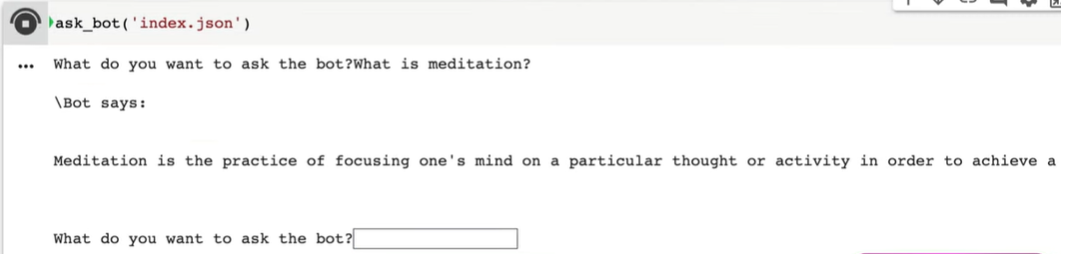
\includegraphics[width=\linewidth,keepaspectratio]{chatgpt42}
\end{center}		


\end{frame}



%%%%%%%%%%%%%%%%%%%%%%%%%%%%%%%%%%%%%%%%%%%%%%%%%%%%%%%%%%%%%%%%%%%%%%%%%%%%%%%%%%
\begin{frame}[fragile]\frametitle{}
\begin{center}
{\Large Customizing GPT-3 for your application - Jsonl method\\ OpenAI}
\end{center}
\end{frame}

%%%%%%%%%%%%%%%%%%%%%%%%%%%%%%%%%%%%%%%%%%%%%%%%%%%%%%%%%%%
\begin{frame}[fragile]\frametitle{Fine tuning}

\begin{itemize}
\item Developers can now fine-tune GPT-3 on their own data
\item Creating a custom version tailored to their application.
\item You can use an existing dataset of virtually any shape and size, or incrementally add data based on user feedback. 
\item With fine-tuning, one API customer was able to increase correct outputs from 83\% to 95\%. 
\item By adding new data from their product each week, another reduced error rates by 50\%.
\end{itemize}	 

\end{frame}

%%%%%%%%%%%%%%%%%%%%%%%%%%%%%%%%%%%%%%%%%%%%%%%%%%%%%%%%%%%
\begin{frame}[fragile]\frametitle{Fine tuning}

Fine-tuning lets you get more out of the models available through the API by providing:

\begin{itemize}
\item Higher quality results than prompt design
\item Ability to train on more examples than can fit in a prompt
\item Token savings due to shorter prompts
\item Lower latency requests
\end{itemize}	 


{\tiny (Ref: https://platform.openai.com/docs/guides/fine-tuning)}
\end{frame}

%%%%%%%%%%%%%%%%%%%%%%%%%%%%%%%%%%%%%%%%%%%%%%%%%%%%%%%%%%%
\begin{frame}[fragile]\frametitle{Fine tuning}

\begin{itemize}
\item GPT-3 has been pre-trained on a vast amount of text from the open Internet. 
\item When given a prompt with just a few examples, it can often intuit what task you are trying to perform and generate a plausible completion. This is often called "few-shot learning."
\item Fine-tuning improves on few-shot learning by training on many more examples than can fit in the prompt, letting you achieve better results on a wide number of tasks. 
\item Once a model has been fine-tuned, you won't need to provide examples in the prompt anymore. 
\item This saves costs and enables lower-latency requests.
\end{itemize}	 


{\tiny (Ref: https://platform.openai.com/docs/guides/fine-tuning)}
\end{frame}

%%%%%%%%%%%%%%%%%%%%%%%%%%%%%%%%%%%%%%%%%%%%%%%%%%%%%%%%%%%
\begin{frame}[fragile]\frametitle{Fine tuning}

Fine-tuning involves the following steps:

\begin{itemize}
\item Prepare and upload training data
\item Train a new fine-tuned model
\item Use your fine-tuned model
\item Pricing below
\end{itemize}	 

\begin{center}
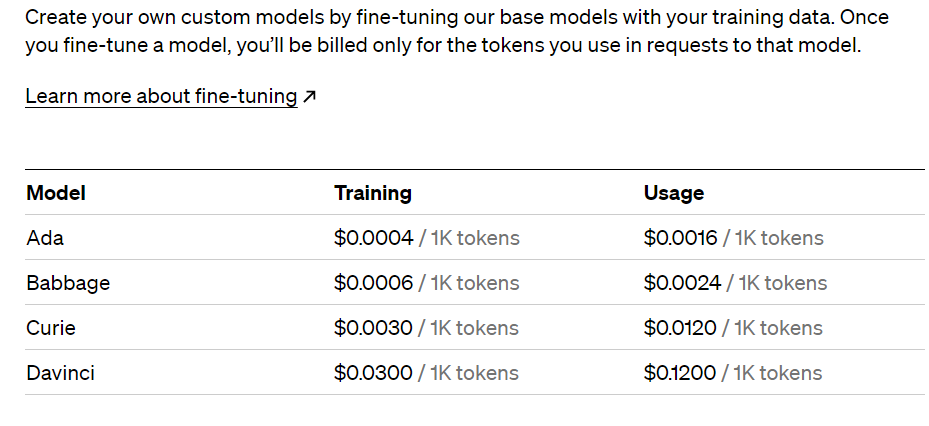
\includegraphics[width=\linewidth,keepaspectratio]{chatgpt41}

{\tiny (Ref: https://openai.com/pricing)}

\end{center}		

\end{frame}

%%%%%%%%%%%%%%%%%%%%%%%%%%%%%%%%%%%%%%%%%%%%%%%%%%%%%%%%%%%
\begin{frame}[fragile]\frametitle{What models can be fine-tuned?}

\begin{itemize}
\item Fine-tuning is currently only available for the following base models: davinci, curie, babbage, and ada. 
\item These are the original models that do not have any instruction following training (like text-davinci-003 does for example). 
\item You are also able to continue fine-tuning a fine-tuned model to add additional data without having to start from scratch.
\end{itemize}	 


{\tiny (Ref: https://platform.openai.com/docs/guides/fine-tuning)}
\end{frame}

%%%%%%%%%%%%%%%%%%%%%%%%%%%%%%%%%%%%%%%%%%%%%%%%%%%%%%%%%%%
\begin{frame}[fragile]\frametitle{Setup}

\begin{lstlisting}
pip install --upgrade openai
OPENAI_API_KEY="<OPENAI_API_KEY>"
\end{lstlisting}	 

\end{frame}

%%%%%%%%%%%%%%%%%%%%%%%%%%%%%%%%%%%%%%%%%%%%%%%%%%%%%%%%%%%
\begin{frame}[fragile]\frametitle{Prepare Training Data}

\begin{itemize}
\item Your data must be a JSONL document, where each line is a prompt-completion pair corresponding to a training example. 
\item You can use our CLI data preparation tool to easily convert your data into this file format.
\end{itemize}	 

\begin{lstlisting}
{"prompt": "<prompt text>", "completion": "<ideal generated text>"}
{"prompt": "<prompt text>", "completion": "<ideal generated text>"}
{"prompt": "<prompt text>", "completion": "<ideal generated text>"}
...
\end{lstlisting}	 

\end{frame}


%%%%%%%%%%%%%%%%%%%%%%%%%%%%%%%%%%%%%%%%%%%%%%%%%%%%%%%%%%%
\begin{frame}[fragile]\frametitle{Prepare Training Data}

\begin{itemize}
\item Designing your prompts and completions for fine-tuning is different from designing your prompts for use with our base models (Davinci, Curie, Babbage, Ada). 
\item In particular, while prompts for base models often consist of multiple examples ("few-shot learning"), for fine-tuning, each training example generally consists of a single input example and its associated output, without the need to give detailed instructions or include multiple examples in the same prompt.
\item The more training examples you have, the better. We recommend having at least a couple hundred examples. 
\item In general, we've found that each doubling of the dataset size leads to a linear increase in model quality.
\item More at https://platform.openai.com/docs/guides/fine-tuning/preparing-your-dataset
\end{itemize}	 


\end{frame}


%%%%%%%%%%%%%%%%%%%%%%%%%%%%%%%%%%%%%%%%%%%%%%%%%%%%%%%%%%%
\begin{frame}[fragile]\frametitle{Prepare Training Data}

\begin{itemize}
\item We developed a tool which validates, gives suggestions and reformats your data: \lstinline|openai tools fine_tunes.prepare_data -f <LOCAL_FILE>|
\item This tool accepts different formats, with the only requirement that they contain a prompt and a completion column/key. 
\item You can pass a CSV, TSV, XLSX, JSON or JSONL file, and it will save the output into a JSONL file ready for fine-tuning, after guiding you through the process of suggested changes.
\end{itemize}	 


\end{frame}


%%%%%%%%%%%%%%%%%%%%%%%%%%%%%%%%%%%%%%%%%%%%%%%%%%%%%%%%%%%
\begin{frame}[fragile]\frametitle{Create a fine-tuned model}

\begin{itemize}
\item Give name of the base model you're starting from (ada, babbage, curie, or davinci).
\item Running the command does several things:
	\begin{itemize}
	\item Uploads the file using the files API (or uses an already-uploaded file)
	\item Creates a fine-tune job
	\item Streams events until the job is done (this often takes minutes, but can take hours if there are many jobs in the queue or your dataset is large)
	\end{itemize}	 
\item Every fine-tuning job starts from a base model, which defaults to curie. 
\item The choice of model influences both the performance of the model and the cost of running your fine-tuned model.
\end{itemize}	 

\begin{lstlisting}
openai api fine_tunes.create -t <TRAIN_FILE_ID_OR_PATH> -m <BASE_MODEL>
\end{lstlisting}	

\end{frame}


%%%%%%%%%%%%%%%%%%%%%%%%%%%%%%%%%%%%%%%%%%%%%%%%%%%%%%%%%%%
\begin{frame}[fragile]\frametitle{Use a fine-tuned model}

\begin{itemize}
\item When a job has succeeded, the \lstinline|fine_tuned_model| field will be populated with the name of the model. You may now specify this model as a parameter to our Completions API, and make requests to it using the Playground.
\item You can start making requests by passing the model name as the model parameter of a completion request:
\end{itemize}	 

\begin{lstlisting}
OpenAI CLI:
openai api completions.create -m <FINE_TUNED_MODEL> -p <YOUR_PROMPT>

Curl:
curl https://api.openai.com/v1/completions \
  -H "Authorization: Bearer $OPENAI_API_KEY" \
  -H "Content-Type: application/json" \
  -d '{"prompt": YOUR_PROMPT, "model": FINE_TUNED_MODEL}'

Python:	
import openai
openai.Completion.create(
    model=FINE_TUNED_MODEL,
    prompt=YOUR_PROMPT)
		
\end{lstlisting}	
		
\end{frame}

%%%%%%%%%%%%%%%%%%%%%%%%%%%%%%%%%%%%%%%%%%%%%%%%%%%%%%%%%%%
\begin{frame}[fragile]\frametitle{Delete a fine-tuned model}

To delete a fine-tuned model, you must be designated an "owner" within your organization.

\begin{lstlisting}
OpenAI CLI:

openai api models.delete -i <FINE_TUNED_MODEL>
cURL:

curl -X "DELETE" https://api.openai.com/v1/models/<FINE_TUNED_MODEL> \
  -H "Authorization: Bearer $OPENAI_API_KEY"
Python:

import openai
openai.Model.delete(FINE_TUNED_MODEL)

\end{lstlisting}	

\end{frame}

%%%%%%%%%%%%%%%%%%%%%%%%%%%%%%%%%%%%%%%%%%%%%%%%%%%%%%%%%%%
\begin{frame}[fragile]\frametitle{Classification Dataset}

Each input in the prompt should be classified into one of the predefined classes. 
\begin{itemize}
\item Use a separator at the end of the prompt, e.g. \lstinline|\n\n###\n\n|. 
\item Choose classes that map to a single token. At inference time, specify  \lstinline|max_tokens=1| since you only need the first token for classification.
\item Ensure that the prompt + completion doesn't exceed 2048 tokens, including the separator
\item Aim for at least  \lstinline|~100| examples per class
\item To get class log probabilities you can specify \lstinline|logprobs=5| (for 5 classes) when using your model
\item Ensure that the dataset used for finetuning is very similar in structure and type of task as what the model will be used for
\end{itemize}	 


\begin{lstlisting}
{"prompt":"Company: BHFF insurance\nProduct: allround insurance\nAd:One stop shop for all your insurance needs!\nSupported:", "completion":" yes"}
{"prompt":"Company: Loft conversion specialists\nProduct: -\nAd:Straight teeth in weeks!\nSupported:", "completion":" no"}
\end{lstlisting}	
\end{frame}


%%%%%%%%%%%%%%%%%%%%%%%%%%%%%%%%%%%%%%%%%%%%%%%%%%%%%%%%%%%
\begin{frame}[fragile]\frametitle{Results}
\begin{lstlisting}
{
  "id": "cmpl-COMPLETION_ID",
  "object": "text_completion",
  "created": 1589498378,
  "model": "YOUR_FINE_TUNED_MODEL_NAME",
  "choices": [  {
      "logprobs": {
        "text_offset": [19],
        "token_logprobs": [-0.03597255],
        "tokens": [" positive"],
        "top_logprobs": [
          {
            " negative": -4.9785037,
            " positive": -0.03597255
          }
        ]
      },
      "text": " positive",
      "index": 0,
      "finish_reason": "length"
    }
  ]
}
\end{lstlisting}		

\end{frame}


%%%%%%%%%%%%%%%%%%%%%%%%%%%%%%%%%%%%%%%%%%%%%%%%%%%%%%%%%%%
\begin{frame}[fragile]\frametitle{Entity extraction Dataset}

\begin{itemize}
\item This is similar to a language transformation task. 
\item To improve the performance, it is best to either sort different extracted entities alphabetically or in the same order as they appear in the original text. 
\item This will help the model to keep track of all the entities which need to be generated in order. The dataset could look as follows:
\end{itemize}	 


\begin{lstlisting}
{"prompt":"<any text, for example news article>\n\n###\n\n", "completion":" <list of entities, separated by a newline> END"}

Example:
{"prompt":"Portugal will be removed from the UK's green travel list from Tuesday, amid rising coronavirus cases and concern over a \"Nepal mutation of the so-called Indian variant\". It will join the amber list, meaning holidaymakers should not visit and returnees must isolate for 10 days...\n\n###\n\n", "completion":" Portugal\nUK\nNepal mutation\nIndian variant END"}
\end{lstlisting}	
\end{frame}

%%%%%%%%%%%%%%%%%%%%%%%%%%%%%%%%%%%%%%%%%%%%%%%%%%%%%%%%%%%
\begin{frame}[fragile]\frametitle{Advanced usage}

You can add a suffix of up to 40 characters to your fine-tuned model name using the suffix parameter.



\begin{lstlisting}
openai api fine_tunes.create -t test.jsonl -m ada --suffix "custom model name"

\end{lstlisting}	
\end{frame}



%%%%%%%%%%%%%%%%%%%%%%%%%%%%%%%%%%%%%%%%%%%%%%%%%%%%%%%%%%%
\begin{frame}[fragile]\frametitle{Advanced usage}


We attach a result file to each job once it has been completed. This results file ID will be listed when you retrieve a fine-tune, and also when you look at the events on a fine-tune. You can download these files:


\begin{lstlisting}
openai api fine_tunes.results -i <YOUR_FINE_TUNE_JOB_ID>
\end{lstlisting}	
\end{frame}




%%%%%%%%%%%%%%%%%%%%%%%%%%%%%%%%%%%%%%%%%%%%%%%%%%%%%%%%%%%
\begin{frame}[fragile]\frametitle{Advanced usage}

We also provide the option of generating additional classification-specific metrics in the results file, such as accuracy and weighted F1 score.



\begin{lstlisting}
# For multiclass classification
openai api fine_tunes.create \
  -t <TRAIN_FILE_ID_OR_PATH> \
  -v <VALIDATION_FILE_OR_PATH> \
  -m <MODEL> \
  --compute_classification_metrics \
  --classification_n_classes <N_CLASSES>

# For binary classification
openai api fine_tunes.create \
  -t <TRAIN_FILE_ID_OR_PATH> \
  -v <VALIDATION_FILE_OR_PATH> \
  -m <MODEL> \
  --compute_classification_metrics \
  --classification_n_classes 2 \
  --classification_positive_class <POSITIVE_CLASS_FROM_DATASET>
\end{lstlisting}	
\end{frame}

%%%%%%%%%%%%%%%%%%%%%%%%%%%%%%%%%%%%%%%%%%%%%%%%%%%%%%%%%%%
\begin{frame}[fragile]\frametitle{Validation}

\begin{itemize}
\item You can reserve some of your data for validation. A validation file has exactly the same format as a train file, and your train and validation data should be mutually exclusive.
\item 
If you include a validation file when creating your fine-tune job, the generated results file will include evaluations on how well the fine-tuned model performs against your validation data at periodic intervals during training.
\end{itemize}


\begin{lstlisting}
openai api fine_tunes.create -t <TRAIN_FILE_ID_OR_PATH> \
  -v <VALIDATION_FILE_ID_OR_PATH> \
  -m <MODEL>
\end{lstlisting}	
\end{frame}

%%%%%%%%%%%%%%%%%%%%%%%%%%%%%%%%%%%%%%%%%%%%%%%%%%%%%%%%%%%
\begin{frame}[fragile]\frametitle{Hyperparameters}

Tweaking the hyperparameters used for fine-tuning can often lead to a model that produces higher quality output. In particular, you may want to configure the following:

\begin{itemize}
\item \lstinline|model|: The name of the base model to fine-tune. You can select one of "ada", "babbage", "curie", or "davinci". To learn more about these models, see the Models documentation.
\item \lstinline|n_epochs| - defaults to 4. The number of epochs to train the model for. An epoch refers to one full cycle through the training dataset.
\item \lstinline|batch_size| - defaults to ~0.2% of the number of examples in the training set, capped at 256. The batch size is the number of training examples used to train a single forward and backward pass. In general, we've found that larger batch sizes tend to work better for larger datasets.
\item \lstinline|learning_rate_multiplier| - defaults to 0.05, 0.1, or 0.2 depending on final batch\_size. The fine-tuning learning rate is the original learning rate used for pretraining multiplied by this multiplier. We recommend experimenting with values in the range 0.02 to 0.2 to see what produces the best results. Empirically, we've found that larger learning rates often perform better with larger batch sizes.
\item \lstinline|compute_classification_metrics| - defaults to False. If True, for fine-tuning for classification tasks, computes classification-specific metrics (accuracy, F-1 score, etc) on the validation set at the end of every epoch.
\end{itemize}


\end{frame}





%%%%%%%%%%%%%%%%%%%%%%%%%%%%%%%%%%%%%%%%%%%%%%%%%%%%%%%%%%%%%%%%%%%%%%%%%%%%%%%%%%
\begin{frame}[fragile]\frametitle{}
\begin{center}
{\Large GPT-3 Alternatives}
\end{center}
\end{frame}

%%%%%%%%%%%%%%%%%%%%%%%%%%%%%%%%%%%%%%%%%%%%%%%%%%%%%%%%%%%
\begin{frame}[fragile]\frametitle{Bloom}

\begin{itemize}
\item Developed by a group of over 1,000 AI researchers
\item Open-source multilingual language model
\item Trained on 176 billion parameters, which is a billion more than GPT-3 
\item Training required 384 graphics cards for training, each having a memory of more than 80 gigabytes.
\end{itemize}	 

\tiny{(Ref: Top 10 Open-Source GTP3 Alternatives You Should Try in 2023 - Apoorva Bellapu)}
\end{frame}

%%%%%%%%%%%%%%%%%%%%%%%%%%%%%%%%%%%%%%%%%%%%%%%%%%%%%%%%%%%
\begin{frame}[fragile]\frametitle{Chinchilla}

\begin{itemize}
\item Developed by DeepMind
\item 70 billion parameters but with four times more data
\item Outperformed Gopher, GPT-3, Jurassic-1, and Megatron-Turing NLG on several downstream evaluation tasks
\item Requires very less computing power for fine tuning and inference.
\end{itemize}	 

\tiny{(Ref: Top 10 Open-Source GTP3 Alternatives You Should Try in 2023 - Apoorva Bellapu)}
\end{frame}

%%%%%%%%%%%%%%%%%%%%%%%%%%%%%%%%%%%%%%%%%%%%%%%%%%%%%%%%%%%
\begin{frame}[fragile]\frametitle{Gopher}

\begin{itemize}
\item Developed by DeepMind
\item 280 billion parameters
\item Has an expertise in answering science and humanities questions much better than other languages.
\end{itemize}	 

\tiny{(Ref: Top 10 Open-Source GTP3 Alternatives You Should Try in 2023 - Apoorva Bellapu)}
\end{frame}

%%%%%%%%%%%%%%%%%%%%%%%%%%%%%%%%%%%%%%%%%%%%%%%%%%%%%%%%%%%
\begin{frame}[fragile]\frametitle{Megatron-Turing Natural Language Generation (NLG)}

\begin{itemize}
\item Developed by NVIDIA and Microsoft
\item 530 billion parameters
\item Trained on the NVIDIA DGX SuperPOD-based Selene supercomputer and is one of the most powerful English language models.
\end{itemize}	 

\tiny{(Ref: Top 10 Open-Source GTP3 Alternatives You Should Try in 2023 - Apoorva Bellapu)}
\end{frame}

%%%%%%%%%%%%%%%%%%%%%%%%%%%%%%%%%%%%%%%%%%%%%%%%%%%%%%%%%%%
\begin{frame}[fragile]\frametitle{PaLM}

\begin{itemize}
\item Developed by Google 
\item 540 billion parameters
\item Has evolved into a dense decoder-only transformer model trained with the Pathways system.
\item Outperformed 28 out of 29 NLP tasks in English when compared to other models.
\end{itemize}	 

\tiny{(Ref: Top 10 Open-Source GTP3 Alternatives You Should Try in 2023 - Apoorva Bellapu)}
\end{frame}

%%%%%%%%%%%%%%%%%%%%%%%%%%%%%%%%%%%%%%%%%%%%%%%%%%%%%%%%%%%
\begin{frame}[fragile]\frametitle{LaMDA}

\begin{itemize}
\item Developed by Google 
\item 137 billion parameters
\item Dataset of 1.5 trillion words which is 40 times more than previously developed models. 
\item Has already been used for zero-shot learning, program synthesis, and BIG-bench workshop.
\end{itemize}	 

\tiny{(Ref: Top 10 Open-Source GTP3 Alternatives You Should Try in 2023 - Apoorva Bellapu)}
\end{frame}

%%%%%%%%%%%%%%%%%%%%%%%%%%%%%%%%%%%%%%%%%%%%%%%%%%%%%%%%%%%
\begin{frame}[fragile]\frametitle{Open Pre-trained Transformer (OPT) }

\begin{itemize}
\item 175 billion parameters
\item Trained on openly available datasets allowing more community engagement. 
\item Comes with the pre-trained models along with code for training.
\item Currently under noncommercial license and available for research use only. 
\end{itemize}	 

\tiny{(Ref: Top 10 Open-Source GTP3 Alternatives You Should Try in 2023 - Apoorva Bellapu)}
\end{frame}



